\documentclass[11pt]{article}
\usepackage[utf8]{inputenc}
\usepackage[a4paper]{geometry}
\usepackage{amsmath}
\usepackage{amssymb}
\usepackage{amsthm}
\usepackage{array}
\usepackage{chngcntr}
\usepackage{commath}
\usepackage{comment}
\usepackage{enumitem}
\usepackage{float}
\usepackage{hyperref}
\usepackage{pgfplots}
\usepackage{stmaryrd}
\usepackage{thmtools}
\usepackage{tikz}
\usepackage{tikz-cd}
\usepackage{titlesec}

\usetikzlibrary{shapes,calc,arrows,through,intersections}
\pgfplotsset{compat=1.18}

\theoremstyle{definition}
\newtheorem{definition}{Definition}[section]
\newtheorem*{definition*}{Definition}
\newtheorem{example}[definition]{Example}
\newtheorem*{example*}{Example}
\newtheorem*{exercise}{Exercise}
\newtheorem*{fact}{Fact}

\theoremstyle{plain}
\newtheorem{theorem}[definition]{Theorem}
\newtheorem{proposition}[definition]{Proposition}
\newtheorem{lemma}[definition]{Lemma}
\newtheorem{corollary}[definition]{Corollary}

\theoremstyle{remark}
\newtheorem{remark}[definition]{Remark}
\newtheorem*{remark*}{Remark}

\renewcommand{\qedsymbol}{$\blacksquare$}

\DeclareMathOperator{\Char}{char}
\DeclareMathOperator{\Gal}{Gal}
\DeclareMathOperator{\id}{id}
\DeclareMathOperator{\area}{area}
\DeclareMathOperator{\ord}{ord}
\DeclareMathOperator{\Frac}{Frac}
\let\div\undefined
\DeclareMathOperator{\div}{div}
\DeclareMathOperator{\Div}{Div}
\DeclareMathOperator{\Pic}{Pic}

\newcommand{\FF}{\mathbb{F}}
\newcommand{\NN}{\mathbb{N}}
\newcommand{\ZZ}{\mathbb{Z}}
\newcommand{\QQ}{\mathbb{Q}}
\newcommand{\RR}{\mathbb{R}}
\newcommand{\CC}{\mathbb{C}}
\newcommand{\PP}{\mathbb{P}}
\newcommand{\bA}{\mathbb{A}}
\newcommand{\cD}{\mathcal{D}}
\newcommand{\cL}{\mathcal{L}}

\setlist[enumerate,1]{label=(\roman*), nosep}
\setlist[itemize,1]{nosep}

% Uncomment to exclude proofs
% \excludecomment{proof}

\title{Part III Elliptic Curves Lecture Notes}
\author{Ming Yean Lim}

\begin{document}

\maketitle

\noindent These lecture notes were based on the Part III course Elliptic Curves taught during Lent 2023 by Professor Tom Fisher.

\tableofcontents

\newcommand{\sectionbreak}{\clearpage}

\section{Fermat's Method of Infinite Descent}

Let $\Delta$ be the right-angled triangle
\begin{center}
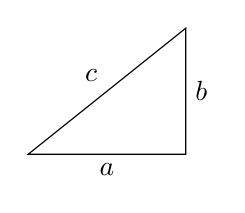
\begin{tikzpicture}[scale=1, transform shape]
    \draw (0,0) -- node[auto, swap]{$a$} (2,0) -- node[auto, swap]{$b$} (2,1.6) -- node[auto, swap]{$c$} cycle;
\end{tikzpicture}
\end{center}
We have $a^2 + b^2 = c^2$, and $\area(\Delta) = \frac{1}{2} a b$.

\begin{definition*}
    We say $\Delta$ is \emph{rational} if $a, b, c \in \QQ$, and $\Delta$ is \emph{primitive} if $a, b, c \in \ZZ$ are coprime\footnote{this is equivalent to $a, b, c$ being pairwise coprime}.
\end{definition*}

\begin{lemma}\label{lem:1_1}
    Every primitive triangle\footnote{we allow swapping edges $a$ and $b$} is of the form
    \begin{center}
    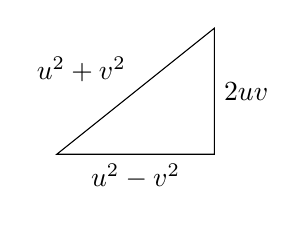
\begin{tikzpicture}[scale=1, transform shape]
        \draw (0,0) -- node[auto, swap]{$u^2 - v^2$} (2,0) -- node[auto, swap]{$2uv$} (2,1.6) -- node[auto, swap]{$u^2 + v^2$} cycle;
    \end{tikzpicture}
    \end{center}
    for some integers $u > v > 0$.
\end{lemma}
\begin{proof}
    $a$ and $b$ cannot be both odd, otherwise $c^2 \equiv 2 \pmod{4}$, which has no solutions. They cannot be both even either, since we are assuming the triangle to be primitive.

    WLOG $a$ is odd and $b$ is even, so that $c$ is odd. Then
    \begin{equation*}
        \left(\frac{b}{2}\right)^2 = \frac{c+a}{2} \frac{c-a}{2}
    \end{equation*}
    is a product of coprime positive integers. Indeed $(\frac{c+a}{2}, \frac{c-a}{2}) \mid (a, c) = 1$. Thus by unique factorisation in $\ZZ$, $\frac{c+a}{2} = u^2$ and $\frac{c-a}{2} = v^2$ for some $u, v \in \ZZ_{>0}$. Then $a = u^2 - v^2$, $b = 2uv$, and $c = u^2 + v^2$.
\end{proof}

\begin{definition*}
    $D \in \QQ_{> 0}$ is a \emph{congruent number} if there exists a rational right-angled triangle with $\area(\Delta) = D$.
\end{definition*}

\noindent To find all congruent numbers, it suffices to consider $D \in \ZZ_{>0}$ squarefree.

\begin{example*}
    $D = 5, 6$ are congruent numbers.
\end{example*}

\begin{lemma}\label{lem:1_2}
    $D \in \QQ_{> 0}$ is a congruent number if and only if $D y^2 = x^3 - x$ for some $x, y \in \QQ$ with $y \neq 0$.
\end{lemma}
\begin{proof}
    \autoref{lem:1_1} shows that $D$ is congruent iff $D w^2 = u v (u^2 - v^2)$ for some $u, v, w \in \QQ$ with $w \neq 0$. Setting $x =\frac{u}{v}$ and $y = \frac{w}{v^2}$ gives the equation in the lemma.
\end{proof}

\begin{theorem}\label{thm:1_3}
    There is no solution to
    \begin{equation}\label{eqn:1_3_star}
        w^2 = u v (u + v) (u - v) \quad \text{ for } u, v, w \in \ZZ, w \neq 0
    \end{equation}
\end{theorem}
\begin{proof}
    Suppose we have a solution $u, v, w$. Dividing out the common factor of $u$ and $v$, we may assume that $u, v$ are coprime. By flipping signs of $u, v$, we may assume that $u > 0$. Clearly we can assume $w > 0$. We can also assume $v > 0$: if $v < 0$, then replace $(u, v, w)$ by $(-v, u, w)$. If $u \equiv v \pmod{2}$, then replace $(u, v, w)$ by $(\frac{u+v}{2}, \frac{u-v}{2}, \frac{w}{2})$.

    Thus $u, v, u+v, u-v$ are pairwise coprime\footnote{$(u+v, u-v) \mid 2(u, v) = 2$, but $u \pm v$ are both odd, so $(u+v, u-v) = 1$} positive integers with their product a square. By unique factorisation in $\ZZ$, $u = a^2$, $v = b^2$, $u+v = c^2$, and $u-v = d^2$ for some $a, b, c, d \in \ZZ_{>0}$. Since $u \not\equiv v \pmod{2}$, $c, d$ are both odd. Then
    \begin{equation*}
        \left(\frac{c+d}{2}\right)^2 + \left(\frac{c-d}{2}\right)^2 = \frac{c^2 + d^2}{2} = u = a^2
    \end{equation*}
    Then
    \begin{center}
    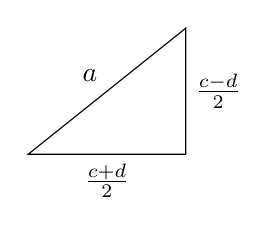
\begin{tikzpicture}[scale=1, transform shape]
        \draw (0,0) -- node[auto, swap]{$\frac{c+d}{2}$} (2,0) -- node[auto, swap]{$\frac{c-d}{2}$} (2,1.6) -- node[auto, swap]{$a$} cycle;
    \end{tikzpicture}
    \end{center}
    is a primitive triangle of area $\frac{c^2 - d^2}{8} = \frac{v}{4} = (\frac{b}{2})^2$. Let $w_1 = \frac{b}{2}$. Let $u_1, v_1 \in \ZZ_{>0}$ be the $u, v$ in \autoref{lem:1_1} corresponding to this triangle. Then $w_1^2 = u_1 v_1 (u_1 + v_1) (u_1 - v_1)$, which gives a new solution to \eqref{eqn:1_3_star}. We have $4 w_1^2 = b^2 = v \mid w^2$ implies $w_1 \le \frac{w}{2}$, so we have a solution with a smaller $w$. By Fermat's method of infinite descent, there is no solution to \eqref{eqn:1_3_star}.
\end{proof}

Now we will see a variant of this for polynomials. In this section , we let $K$ be a field with $\Char K \neq 2$, and $\overline{K}$ its algebraic closure.

\begin{lemma}\label{lem:1_4}
    Let $u, v \in K[t]$ be coprime. If $\alpha u + \beta v$ is a square for 4 distinct $(\alpha : \beta) \in \PP^1$, then $u, v \in K$.
\end{lemma}
\begin{proof}
    WLOG $K = \overline{K}$ is algebraically closed. By changing coordinates\footnote{$u, v$ are replaced by an invertible linear combination} on $\PP^1$, we may assume that the ratios $(\alpha : \beta)$ are $(1 : 0), (0 : 1), (1 : -1), (1 : -\lambda)$ for some $\lambda \in K \setminus \{0,1\}$.
    \begin{align*}
        u &= a^2\\
        v &= b^2\\
        u-v &= (a+b)(a-b)\\
        u-\lambda v &= (a+\mu b)(a-\mu b)
    \end{align*}
    for some $a, b \in K[t]$, and $\mu = \sqrt{\lambda}$. By unique factorisation in $K[t]$, $a+b, a-b, a+\mu b, a-\mu b$ are squares. But\footnote{$\max\{\deg{u}, \deg{v}\}$ does not change when we replace $u, v$ with an invertible linear combination} $\max\{\deg{a}, \deg{b}\} \le \frac{1}{2} \max\{\deg{u}, \deg{v}\}$, so by Fermat's method of infinite descent, $u, v \in K$.
\end{proof}

\begin{definition}\label{def:1_5}\phantom{}
    \begin{enumerate}
        \item An \emph{elliptic curve} $E/K$ is the projective closure of the plane affine curve
            \begin{equation}\label{eqn:weierstrass_eqn}
                y^2 = f(x)
            \end{equation}
            where $f \in K[x]$ is a monic cubic polynomial with distinct roots in $\overline{K}$. \eqref{eqn:weierstrass_eqn} is called a \emph{Weierstrass equation}.

        \item For $L/K$ a field extension, set $E(L) = \{(x, y) \in L \mid y^2 = f(x)\} \cup \{0\}$, where $0$ denotes the point at infinity.
    \end{enumerate}
\end{definition}

\begin{fact}
    $E(L)$ is naturally an abelian group.
\end{fact}

In this course we will study $E(K)$ for $K$ a finite field, local field ($[K : \QQ_p] < \infty$), and number field.

\autoref{lem:1_2} and \autoref{thm:1_3} imply that for $E : y^2 = x^3 - x$, we have $E(\QQ) = \{0, (0, 0), (\pm 1, 0)\}$. As we will see, this is a group isomorphic to $C_2 \times C_2$.

\begin{corollary}\label{cor:1_6}
    Let $E/K$ be an elliptic curve. Then $E(K(t)) = E(K)$.
\end{corollary}
\begin{proof}
    WLOG $K = \overline{K}$ is algebraically closed. By a change of coordinates, we may assume that
    \begin{equation*}
        E : y^2 = x(x-1)(x-\lambda)
    \end{equation*}
    for some $\lambda \in K \setminus \{0, 1\}$

    Suppose that $(x, y) \in E(K(t))$. Write $x = \frac{u}{v}$, where $u, v \in K[t]$ are coprime. Then $w^2 = uv(u-v)(u-\lambda v)$ for some $w \in K[t]$. Unique factorisation in $K[t]$ implies that $u, v, u-v, u-\lambda v$ are all squares.\footnote{we can absorb constants since $K$ is algebraically closed} \autoref{lem:1_4} then implies that $u, v \in K$, so $x, y \in K$.
\end{proof}

\section{Some Remarks on Algebraic Curves}

In this section we will work over an algebraically closed field $K = \overline{K}$.

\begin{definition}\label{def:2_1}
    A plane curve $C = \{f(x, y) = 0\} \subseteq \bA^2$ (with $f \in K[x, y]$ irreducible) is \emph{rational} if it has a \emph{rational parameterisation}, i.e. there exists $\phi, \psi \in K(t)$ such that
    \begin{enumerate}
        \item The map $\bA^2 \to \bA^2$ defined by $t \mapsto (\phi(t), \psi(t))$ is injective on $\bA^1 \setminus \{\text{finite set}\}$.
        \item $f(\phi(t), \psi(t)) = 0$.
    \end{enumerate}
\end{definition}

\begin{example}\label{eg:2_2}\phantom{}
    \begin{enumerate}[label=(\alph*)]
        \item Any nonsingular plane conic is rational. We illustrate the proof of this with the unit circle:
            \begin{figure}[H]
            \centering
            \scalebox{0.8}{
            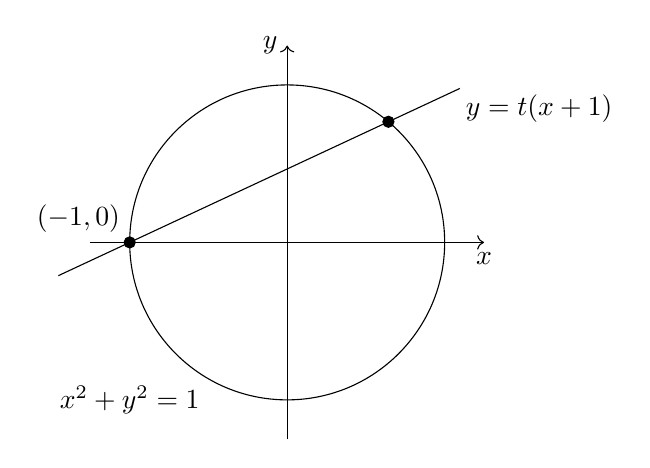
\begin{tikzpicture}
                \coordinate (A) at (-2,0);
                \coordinate (B) at ({2*cos(50)}, {2*sin(50)});

                \draw[name path=Circle] (0,0) circle (2);
                \draw[->] (-2.5,0) -- (2.5,0) node[below] {$x$};
                \draw[->] (0,-2.5) -- (0,2.5) node[left] {$y$};
                \draw[shorten >= -1cm, shorten <= -1cm, name path=Line] (A) -- (B);

                \filldraw[black] (A) circle (2pt) node[above left] {$(-1, 0)$} (B) circle (2pt);
                \node at (-2, -2) {$x^2+y^2=1$};
                \node at (3.2, 1.7) {$y=t(x+1)$};
            \end{tikzpicture}}
            \end{figure}
            We choose a point on the conic, here we take $(-1, 0)$. Then draw a line of slope $t$ through the point, $y = t(x+1)$. Solving for the other intersection point, we have $x^2 + t^2 (x+1)^2$, which implies $(x+1)(x-1+t^2(x+1)) = 0$. Thus $(x, y) = (\frac{1-t^2}{1+t^2}, \frac{2t}{1+t^2})$ gives a rational parameterisation.

        \item Any singular plane cubic is rational. We apply the same procedure as before, but we choose the singular point instead of an arbitrary point.
            \begin{figure}[H]
            \centering
            \begin{minipage}{.5\textwidth}
            \centering
            \scalebox{0.8}{
            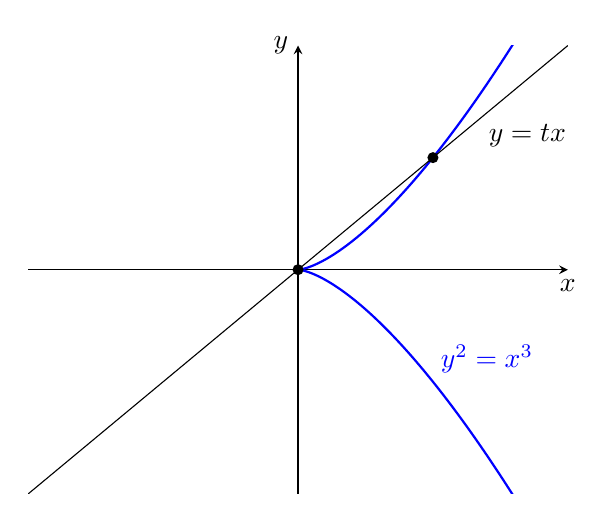
\begin{tikzpicture}[scale=1, transform shape]
                \begin{axis}[
                    axis lines=middle,
                    xlabel=$x$,
                    ylabel=$y$,
                    xtick=\empty,
                    ytick=\empty,
                    xmin=-2, xmax=2,
                    ymin=-2, ymax=2,
                    xlabel style={anchor=north},
                    ylabel style={anchor=east},
                    samples=100,
                    ]
                \addplot[thick,domain=0:2, name path=curve, blue] {sqrt(x^3)};
                \addplot[thick,domain=0:2, blue] {-sqrt(x^3)};
                \addplot[domain=-2:2, name path=line] {1*x};
                \fill [name intersections={of=curve and line,by={a,b}}] (a) circle[radius=2pt] (b) circle[radius=2pt];
                \node[blue] at (axis cs:1.4,-0.8) {$y^2=x^3$};
                \node at (axis cs:1.7,1.2) {$y=tx$};
                \end{axis}
            \end{tikzpicture}}
            \end{minipage}%
            \begin{minipage}{.5\textwidth}
            \centering
            \scalebox{0.8}{
            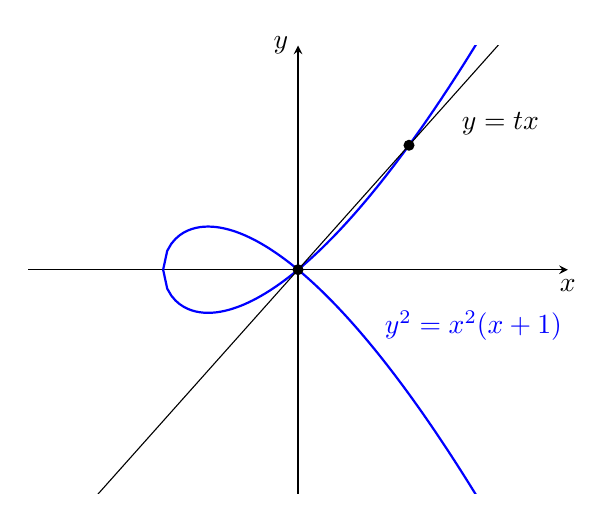
\begin{tikzpicture}[scale=1, transform shape]
                \begin{axis}[
                    axis lines=middle,
                    xlabel=$x$,
                    ylabel=$y$,
                    xtick=\empty,
                    ytick=\empty,
                    xmin=-2, xmax=2,
                    ymin=-2, ymax=2,
                    xlabel style={anchor=north},
                    ylabel style={anchor=east},
                    samples=100,
                    ]
                \addplot[thick,domain=-1:2, name path=curve, blue] {x*sqrt(x+1)};
                \addplot[thick,domain=-1:2, blue] {-x*sqrt(x+1)};
                \addplot[domain=-2:2, name path=line] {1.35*x};
                \fill [name intersections={of=curve and line,by={a,b}}] (a) circle[radius=2pt] (b) circle[radius=2pt];
                \node[blue] at (axis cs:1.3,-0.5) {$y^2=x^2(x+1)$};
                \node at (axis cs:1.5,1.3) {$y=tx$};
                \end{axis}
            \end{tikzpicture}}
            \end{minipage}
            \end{figure}
            The curve on the left has parameterisation $(x,y)=(t^2,t^3)$. The parameterisation of the other curve is left as an exercise. Note that these are not elliptic curves.

        \item \autoref{cor:1_6} shows that elliptic curves are not rational.
    \end{enumerate}
\end{example}

\begin{remark}\label{rem:2_3}
    The genus $g(C) \in \ZZ_{\ge 0}$ is an invariant of a smooth projective curve $C$.
    \begin{enumerate}
        \item If $K = \CC$, then $g(C)$ is the genus of the Riemann surface.
        \item A smooth plane curve $C \subseteq \PP^2$ of degree $d$ has genus $g(C) = \frac{(d-1)(d-2)}{2}$.
    \end{enumerate}
\end{remark}

\begin{proposition}\label{prop:2_4}
    Let $C$ be a smooth projective curve.
    \begin{enumerate}
        \item $C$ is rational (see \autoref{def:2_1}) iff $g(C) = 0$;
        \item $C$ is an elliptic curve (see \autoref{def:1_5}) iff $g(C) = 1$.
    \end{enumerate}
\end{proposition}
\begin{proof}\phantom{}
    \begin{enumerate}
        \item Omitted.

        \item ($\Rightarrow$) See Example Sheet and \autoref{rem:2_3}.

            ($\Leftarrow$) We will see this later. \qedhere
    \end{enumerate}
\end{proof}

\subsection*{Order of Vanishing}

Let $C$ be an algebraic curve, $K(C)$ its function field, and $P \in C$ a smooth point. We write $\ord_P(f)$ for the order of vanishing of $f \in K(C)$ at $P$. This is negative if $f$ has a pole at $P$.

\begin{fact}
    $\ord_P : K(C)^\times \to \ZZ$ is a discrete valuation, i.e. $\ord_P(f_1 f_2) = \ord_P(f_1) \ord_P(f_2)$, and $\ord_P(f_1 + f_2) \ge \min(\ord_P(f_1), \ord_P(f_2))$.
\end{fact}

\begin{definition*}
    $t \in K(C)^\times$ is a \emph{uniformiser} at $P$ if $\ord_P(t) = 1$.
\end{definition*}

\begin{example}\label{eg:2_5}
    Let $C = \{g = 0\} \subseteq \bA^2$, with $g \in k[x,y]$ irreducible. Then $K(C) = \Frac \frac{k[x,y]}{(g)}$. Write $g = g_0 + g_1(x,y) + g_2(x,y) + \ldots$, where $g_i$ is homogeneous of degree $i$. Suppose that $P = (0, 0) \in C$ is a smooth point, i.e. $g_0 = 0$, and $g_1(x,y) = \alpha x + \beta y$ with $\alpha, \beta$ not both zero.
    \begin{figure}[htpb]
    \centering
    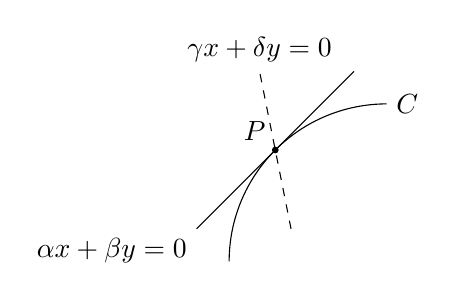
\begin{tikzpicture}[scale=1, transform shape]
        \coordinate (O) at (0,0);
        \draw (O) arc (135:90:2) node[right] {$C$};
        \draw (O) arc (135:180:2);
        \draw (-1,-1) node[below left] {$\alpha x + \beta y = 0$} -- (1,1);
        \filldraw (O) circle (1pt) node[above left] {$P$};
        \draw[dashed] (0.2,-1) -- (-0.2,1) node[above] {$\gamma x + \delta y = 0$};
    \end{tikzpicture}
    \end{figure}

    Let $\gamma, \delta \in K$. Then

    \begin{fact}
        $\gamma x + \delta y \in K(C)$ is a uniformiser at $P$ iff $\alpha \delta - \beta \gamma \neq 0$.
    \end{fact}
\end{example}

\begin{example}\label{eg:2_6}
    Consider the curve $C = \{y^2 = x(x-1)(x-\lambda)\} \subseteq \bA^2$ with $\lambda \neq 0, 1$. Setting $x=X/Z, y=Y/Z$, we get its projective closure $\overline{C} = \{Y^2 Z = X (X-Z) (X-\lambda Z)\} \subseteq \PP^2$. Let $P = (0 : 1 : 0) \in \overline{C}$. Let's compute $\ord_P(x)$ and $\ord_P(y)$.

    Set $t=X/Y, w=Z/Y$. The curve becomes
    \begin{equation}\label{eqn:2_6_star}
        w = t(t-w)(t-\lambda w)
    \end{equation}
    and $P$ is the point $(t,w)=(0,0)$. By looking at the linear part of \eqref{eqn:2_6_star}, we see that $P$ is a smooth point with tangent $w = 0$. By the fact above, $\ord_P(t)=\ord_P(t-w)=\ord_P(t-\lambda w)=1$. Thus \eqref{eqn:2_6_star} implies that $\ord_P(w) = 3$. Then
    \begin{gather*}
        \ord_P(x) = \ord_P\left(\frac{X}{Z}\right) = \ord_P\left(\frac{t}{w}\right) = 1-3 = -2\\
        \ord_P(y) = \ord_P\left(\frac{Y}{Z}\right) = \ord_P\left(\frac{1}{w}\right) = -3
    \end{gather*}
\end{example}

\subsection*{Riemann-Roch Spaces}

Let $C$ be a smooth projective curve.

\begin{definition*}
    A \emph{divisor} is a formal sum of points on $C$, say $C = \sum_{p \in C} n_P P$, with $n_P \in \ZZ$, and $n_P = 0$ for all but finitely many $P \in C$. We let $\Div(C)$ denote the set of divisors. We define $\deg D = \sum_{P \in C} n_P$. $D$ is called \emph{effective} (written $D \ge 0$) if $n_P \ge 0$ for all $P \in C$. If $f \in K(C)^\times$, then define\footnote{$f$ has only finitely many zeros and poles} $\div(f) = \sum_{P \in C} \ord_P(f) P$. The \emph{Riemann-Roch space} of $D \in \Div(C)$ is
    \begin{equation*}
        \cL(D) = \{f \in K(C)^\times \mid \div(f) + D \ge 0\} \cup \{0\}
    \end{equation*}
    i.e. the $K$-vector space of rational functions on $C$ with ``poles no worst than specified by $D$''.
\end{definition*}

We quote the Riemann-Roch Theorem for genus $1$ curves:
\begin{equation*}
    \dim \cL(D) =
    \begin{cases}
        \deg D &\text{if } \deg D > 0\\
        0 \text{ or } 1 &\text{if } \deg D = 0\\
        0 &\text{if } \deg D < 0
    \end{cases}
\end{equation*}

\autoref{eg:2_6} shows that $E : y^2 = f(x)$ and $P$ is the point at infinity, then $\cL(2P) = \langle 1,x \rangle$, and $\cL(3P) = \langle 1,x,y \rangle$.

\begin{proposition}\label{prop:2_7}
    Let $C$ be a smooth plane cubic and $P \in C$ a point of inflection. Then we may change coordinates such that
    \begin{equation*}
        C : Y^2 Z = X (X-Z) (X-\lambda Z)
    \end{equation*}
    for some $\lambda \neq 0, 1$, such that $P = (0:1:0)$.
\end{proposition}
\begin{proof}
    We choose coordinates such that $P = (0:1:0)$ and the tangent line to $C$ at $p$ is $T_p(C) = \{z=0\}$. Write $C = \{F(X,Y,Z) = 0\} \subseteq \PP^2$, where $F$ is a homogeneous cubic polynomial.

    Since $P \in C$ is a point of inflection, $F(t,1,0) = \text{const} \cdot t^3$, hence $F$ has no terms $X^2Y, XY^2, Y^3$, so
    \begin{equation*}
        F \in \langle Y^2Z, XYZ, YZ^2, X^3, X^2Z, XZ^2, Z^3 \rangle
    \end{equation*}
    The coefficient of $Y^2 Z$ is nonzero, otherwise $P \in C$ is a singular point\footnote{by considering the tangent line}. The coefficient of $X^3$ is nonzero, otherwise $\{z = 0\} \subseteq C$. Moreover, we are free to rescale $X,Y,Z$ and $F$. WLOG $C$ is defined by
    \begin{equation}\label{eqn:weierstrass_form}
        C : Y^2 Z + a_1 XYZ + a_3 Y Z^2 = X^3 + a_2 X^2 Z + a_4 X Z^2 + a_6 Z^3
    \end{equation}
    Substituting\footnote{completing the square} $Y \leftarrow Y - \frac{1}{2} a_1 X - \frac{1}{2} a_3 Z$, we may assume $a_1 = a_3 = 0$. Now $C : Y^2 Z = Z^3 f(\frac{X}{Z})$ for some monic cubic polynomial $f$. Since $C$ is smooth, $f$ has distinct roots. By changing coordinates, we may assume the roots are $0, 1, \lambda$. Then
    \begin{equation}\label{eqn:legendre_form}
        C : Y^2 Z = X(X-Z)(X-\lambda Z)
    \end{equation}
    as required.
\end{proof}
\noindent\eqref{eqn:weierstrass_form} is known as a \emph{Weierstrass form} and \eqref{eqn:legendre_form} a \emph{Legendre form}.

\begin{remark*}
    It may be shown that the points of inflection on $C = \{F(X_1, X_2, X_3) = 0\} \subseteq \PP^2$ are given by
    \begin{equation*}
        F = \det \bigg(\md{F}{2}{X_i}{}{X_j}{}\bigg) = 0
    \end{equation*}
\end{remark*}

\subsection*{The Degree of a Morphism}

Let $\phi : C_1 \to C_2$ be a nonconstant morphism of smooth projective curves. Then define $\phi^* : K(C_2) \hookrightarrow K(C_1)$ by $f \mapsto f \circ \phi$. This is an inclusion of fields. We have the tower of fields
\begin{equation*}
\begin{tikzcd}
    K(C_1) \arrow[d, dash]\\
    \phi^*(K(C_2))
\end{tikzcd}
\end{equation*}
we will omit $\phi^*$ if it is clear from the context.

\begin{definition*}\phantom{}
    \begin{enumerate}
        \item $\deg \psi = [K(C_1) : \phi^*(K(C_2))]$.
        \item $\phi$ is \emph{separable} if $K(C_1)/\phi^*(K(C_2))$ is a separable field extension.
    \end{enumerate}
\end{definition*}

\begin{definition*}
    Suppose $P \in C_1$, $Q = \phi(P) \in C_2$. Let $t \in K(C_2)$ be a uniformiser at $Q$. We define $e_\phi(P) = \ord_P(\phi^*(t))$. This is always at least $1$, and is independent of the choice of $t$.
\end{definition*}

\begin{theorem}\label{thm:2_8}
    Let $\phi : C_1 \to C_2$ be a nonconstant morphism of smooth projective curves. Then
    \begin{equation*}
        \sum_{P \in \phi^{-1}(Q)} e_\phi(P) = \deg \phi
    \end{equation*}
    for all $Q \in C_2$. Moreover if $\phi$ is separable, then $e_\phi(P) = 1$ for all but finitely many $P \in C_1$. In particular,
    \begin{enumerate}
        \item $\phi$ is surjective (on $\overline{K}$-points);
        \item $\# \phi^{-1}(Q) \le \deg \phi$;
        \item If $\phi$ is separable, then equality holds in (ii) for all but finitely many $Q \in C_2$.
    \end{enumerate}
\end{theorem}

\begin{remark}\label{rem:2_9}
    Let $C$ be an algebraic curve. A rational map is given by
    \begin{alignat*}{3}
        \phi : C &\dashrightarrow\,\,&& \PP^n\\
        P &\longmapsto&& (f_0(P) : f_1(P) : \ldots : f_n(P))
    \end{alignat*}
    where $f_0, f_1, \ldots, f_n \in K(C)$ are not all zero.
\end{remark}
\begin{fact}
    If $C$ is smooth, then $\phi$ is a morphism.
\end{fact}

\section{Weierstrass Equations}

In this section we will assume that $K$ is a perfect field with algebraic closure $\overline{K}$.

\begin{definition*}
    An \emph{elliptic curve} $E/K$ is a smooth projective curve of genus $1$ defined over $K$, with a specified $K$-rational point $O_E$.
\end{definition*}

\begin{theorem}\label{thm:3_1}
    Every elliptic curve $E$ is isomorphic over $K$ to a curve in Weierstrass form via an isomorphism taking $O_E$ to $(0:1:0)$.
\end{theorem}

\begin{remark*}
    \autoref{prop:2_7} treated the special case $E$ is a smooth plane cubic and $O_E$ is a point of inflection.
\end{remark*}

\begin{fact}
    If $D \in \Div(K)$ is defined over $K$ (i.e. fixed by $\Gal(\overline{K}/K)$), then $\cL(D)$ has a basis in $K(E)$, not just $\overline{K}(E)$.
\end{fact}

\begin{proof}[Proof of \autoref{thm:3_1}]
    $\dim \cL(2 \cdot O_E) = 2$ by the Riemann-Roch theorem, and $1 \in \cL(2 \cdot O_E)$, so we can extend it to a basis $1, x$ of $\cL(2 \cdot O_E)$. We have $\ord_{O_E}(x) = -2$, otherwise $1, x \in \cL(1 \cdot O_E)$. Then we extend it to a basis $1,x,y$ of $\cL(3 \cdot O_E)$, and similarly as before, $\ord_{O_E}(y) = -3$.

    The $7$ elements $1,x,y,x^2,xy,x^3,y^2$ lie in the $6$-dimensional vector space $\cL(6 \cdot O_E)$, so they satisfy a dependence relation. Leaving out $x^3$ or $y^2$ gives a basis of $\cL(6 \cdot O_E)$, since each term has a different order of pole at $O_E$. Thus the coefficients of $x^3$ and $y^2$ in the relation are non-zero. Rescaling $x$ and $y$, we get
    \begin{equation*}
        E' : y^2 + a_1xy + a_3 y = x^3 + a_2x^2 + a_4x + a_6
    \end{equation*}
    for some $a_i \in K$. Let $E'$ be the curve defined by this equation (or rather its projective closure). There is a morphism\footnote{recall that any rational map from a smooth curve is a morphism}
    \begin{alignat*}{3}
        \phi : E &\longrightarrow\,\,&& E'\\
        P &\longmapsto&& (x(P) : y(P) : 1)\\
        & &&= \left(\frac{x}{y}(P) : 1 : \frac{1}{y}(P)\right)\\
        O_E &\longmapsto&& (0 : 1 : 0)
    \end{alignat*}
    We have $\deg \phi = [K(E) : \phi^*(K(E))] = [K(E) : K(x,y)]$.
    \begin{equation*}
        \begin{tikzcd}[column sep=small]
        & K(E) \arrow[d, equal] \arrow[ddl, dash, bend right, "2"'] \arrow[ddr, dash, bend left, "3"] &\\
        & K(x,y) \arrow[dl, dash] \arrow[dr, dash] &\\
        K(x) & & K(y)
    \end{tikzcd}
    \end{equation*}
    Since $x$ was chosen to have a pole of order $2$ at $O_E$ and no other poles, by considering the fibre at $\infty$, we have
    \begin{equation*}
        [K(E) : K(x)] = \deg(E \xrightarrow{x} \PP^1) = \ord_P\left(\frac{1}{x}\right) = 2
    \end{equation*}
    Similarly,
    \begin{equation*}
        [K(E) : K(y)] = \deg(E \xrightarrow{y} \PP^1) = \ord_P\left(\frac{1}{y}\right) = 3
    \end{equation*}
    The tower law implies $\deg \phi = [K(E) : K(x,y)] = 1$. Thus $\phi$ is birational. If $E'$ is singular, then $E$ and $E'$ would be rational, contradiction. Thus $E'$ is smooth, so $\phi^{-1}$ is a morphism. Thus $\phi$ is an isomorphism.
\end{proof}

We say that two elliptic curves are \emph{isomorphic} if they are isomorphic as projective curves with the isomorphism taking specified point to specified point.

\begin{proposition}\label{prop_3_2}
    Let $E, E'$ be elliptic curves over $K$ in Weierstrass form. Then $E \cong E'$ over $K$ iff the equations are related by a change of variables
    \begin{align*}
        x &= u^2 x' + r\\
        y &= u^3 y' + u^2 s x' + t
    \end{align*}
    for some $u,r,s,t \in K$, $u \neq 0$.
\end{proposition}
\begin{proof}
    We have $\langle 1,x \rangle = \cL(2 \cdot O_E) = \langle 1, x' \rangle$ implies that $x = \lambda x' + r$ for some $\lambda, r \in K$, $\lambda \neq 0$. Similarly, $\langle 1,x,y \rangle = \cL(3 \cdot O_E) = \langle 1,x',y' \rangle$ implies $y = \mu y' + \sigma x' + t$ for some $\mu, \sigma, t \in K$, $\mu \neq 0$. Looking at the coefficients of $x^3$ and $y^2$, we see that $\mu^2 = \lambda^3$, so $\lambda = u^2$ and $\mu = u^3$ for some $u \neq 0$. Set $s = \frac{\sigma}{u^2}$
\end{proof}

A Weierstrass equation defines an elliptic curve iff\footnote{for the converse, recall that smooth plane cubics have genus $1$, and we have the specified point $(0:1:0)$} it defines a smooth curve iff $\Delta(a_1, a_2, a_3, a_4, a_6) \neq 0$, where $\Delta \in \ZZ[a_1, a_2, a_3, a_4, a_6]$ is a certain polynomial known as the discriminant. If $\Char K \neq 2, 3$, we can reduce to the case
\begin{equation*}
    E : y^2 = x^3 + a x + b
\end{equation*}
which has discriminant $\Delta = -16(4a^3 + 27b^2)$.

\begin{corollary}
    Assume $\Char K \neq 2, 3$. The elliptic curves
    \begin{gather*}
        E : y^2 = x^3 + ax + b\\
        E' : y^2 = x^3 + a'x + b'
    \end{gather*}
    are isomorphic over $K$ iff $(a',b') = (u^4 a, u^6 b)$ for some $u \in K^\times$.
\end{corollary}
\begin{proof}
    $E$ and $E'$ are related by a substitution as in \autoref{prop_3_2} with $r = s = t = 0$ (simply substitute and expand, using that $a_1 = a_2 = a_3 = 0$).
\end{proof}

\begin{definition*}
    The \emph{$j$-invariant} of $E$ is
    \begin{equation*}
        j(E) = \frac{1728(4a^3)}{4a^3 + 27 b^2}
    \end{equation*}
\end{definition*}

\begin{corollary}\label{cor:3_4}
    If $E \cong E'$, then $j(E) = j(E')$. If $K = \overline{K}$, then the converse holds.
\end{corollary}
\begin{proof}
    We assume $\Char K \neq 2,3$. Then
    \begin{align*}
        E \cong E'
        \iff& (a', b') = (u^4 a, u^6 b) \text{ for some } u \in K^\times\\
        \implies& (a^3 : b^2) = ((a')^3 : (b')^2)\\
        \iff& j(E) = j(E')
    \end{align*}
    and the converse holds if $K = \overline{K}$.
\end{proof}

\section{The Group Law}

Let $E \subseteq \PP^2$ be a smooth plane cubic\footnote{$E = E(\overline{K})$}. Let $P, Q \in E$. $E$ meets any line in $3$ points counted with multiplicity. Set $S$ to be the third point of intersection of $E$ and $PQ$, and $R$ the third point of intersection of $E$ and $O_E S$. Define $P \oplus Q = R$. If $P = Q$, we take $T_P E$ instead of $PQ$, etc. This is called ``the chords and tangent process.''

\begin{figure}[H]
\centering
\scalebox{0.8}{
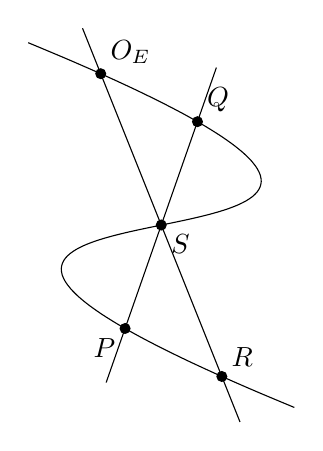
\begin{tikzpicture}[scale=1, transform shape]
    \draw[rotate=75, name path=cubic] plot[variable=\t,domain=-3.6:3.6,smooth,samples=51] ({\t/2}, {\t^3/8 - \t});
    \draw[name path=line1] (-1,2.5) -- (1,-2.5);
    \draw[name path=line2] (0.7,2) -- (-0.7,-2);
    \fill [name intersections={of=cubic and line1,by={r,s,o}}] (r) circle[radius=2pt] node[above right] {$R$} (s) circle[radius=2pt] node[below right] {$S$} (o) circle[radius=2pt] node[above right] {$O_E$};
    \fill [name intersections={of=cubic and line2,by={p,s,q}}] (p) circle[radius=2pt] node[below left] {$P$} (q) circle[radius=2pt] node[above right] {$Q$};
\end{tikzpicture}}
\end{figure}

\begin{theorem}\label{thm:4_1}
    $(E, \oplus)$ is an abelian group.
\end{theorem}
\begin{proof}\phantom{}
    \begin{enumerate}
        \item $\oplus$ is commutative as the order of $P$ and $Q$ did not matter in the construction.

        \item $O_E$ is the identity: Applying the construction, we see that $O_E \oplus P = P$.
            \begin{figure}[H]
            \centering
            \scalebox{0.8}{
            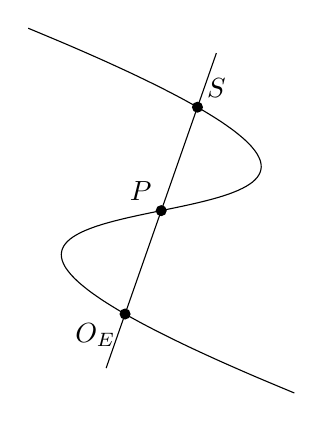
\begin{tikzpicture}[scale=1, transform shape]
                \draw[rotate=75, name path=cubic] plot[variable=\t,domain=-3.6:3.6,smooth,samples=51] ({\t/2}, {\t^3/8 - \t});
                \draw[name path=line2] (0.7,2) -- (-0.7,-2);
                \fill [name intersections={of=cubic and line2,by={o,p,s}}] (o) circle[radius=2pt] node[below left] {$O_E$} (p) circle[radius=2pt] node[above left] {$P$} (s) circle[radius=2pt] node[above right] {$S$};
            \end{tikzpicture}}
            \end{figure}

        \item Inverses: %TODO: Later

        \item Associativity: This is much harder.
    \end{enumerate}
    \renewcommand{\qedsymbol}{}
\end{proof}

\begin{definition*}
    $D_1, D_2 \in \Div(E)$ are \emph{linearly equivalent} if there exists $f \in \overline{K}(E)$ such that $\div(f) = D_1 - D_2$. In this case, we write $D_1 \sim D_2$ and $[D] = \{D' \mid D \sim D'\}$.
\end{definition*}

\begin{definition*}
    The \emph{Picard group} is $\Pic(E) = \Div(E)/\sim$ and $\Pic^0(E) = \Div^0(E)/\sim$, where $\Div^0(E) = \{D \in \Div(E) \mid \deg D = 0\}$.
\end{definition*}

We define
\begin{alignat*}{3}
    \psi : E &\longrightarrow\,\,&& \Pic^0(E)\\
    P &\longmapsto&& [(P) - (O_E)]
\end{alignat*}

\begin{proposition}\label{prop:4_2}\phantom{}
    \begin{enumerate}
        \item $\psi(P \oplus Q) = \psi(P) + \psi(Q)$;
        \item $\psi$ is a bijection.
    \end{enumerate}
\end{proposition}

\begin{proof}\phantom{}
    \begin{enumerate}
        \item Let $l, m \in K(E)$ be as shown below:
            \begin{figure}[H]
            \centering
            \scalebox{0.8}{
            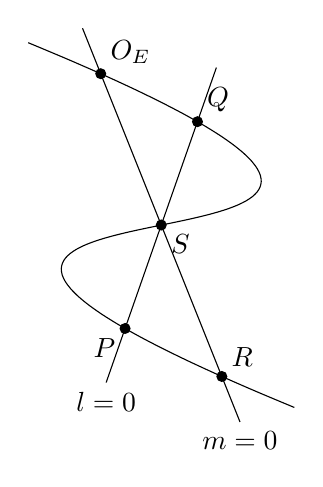
\begin{tikzpicture}[scale=1, transform shape]
                \draw[rotate=75, name path=cubic] plot[variable=\t,domain=-3.6:3.6,smooth,samples=51] ({\t/2}, {\t^3/8 - \t});
                \draw[name path=line1] (-1,2.5) -- (1,-2.5) node[below] {$m = 0$};
                \draw[name path=line2] (0.7,2) -- (-0.7,-2) node[below] {$l = 0$};
                \fill [name intersections={of=cubic and line1,by={r,s,o}}] (r) circle[radius=2pt] node[above right] {$R$} (s) circle[radius=2pt] node[below right] {$S$} (o) circle[radius=2pt] node[above right] {$O_E$};
                \fill [name intersections={of=cubic and line2,by={p,s,q}}] (p) circle[radius=2pt] node[below left] {$P$} (q) circle[radius=2pt] node[above right] {$Q$};
            \end{tikzpicture}}
            \end{figure}
            Then
            \begin{align*}
                \div(l/m)
                &= (P) + (S) + (Q) - (O_E) - (S) - (R)\\
                &= (P) + (Q) - (O_E) - (P \oplus Q)
            \end{align*}
            Thus
            \begin{gather*}
                (P) + (Q) \sim (P \oplus Q) + (O_E)\\
                (P \oplus Q) - (O_E) \sim (P) - (O_E) + (Q) - (O_E)\\
                \psi(P \oplus Q) = \psi(P) + \psi(Q)
            \end{gather*}
            as required.

        \item Next time. \qedhere
    \end{enumerate}
\end{proof}

\end{document}
